\documentclass[11pt]{article}
\usepackage[margin=0.85in]{geometry}
\usepackage{amsmath,amssymb,graphicx,hyperref}
\setlength{\parindent}{0pt}\setlength{\parskip}{6pt}
\setlength{\emergencystretch}{3em}
\begin{document}
{\Large Faithful coordinates and the actual branch radical}\\
November 13, 2026. Symbolic finite transfer [pcc:unverified].

\textbf{Actual coordinate map.} Let $e$ be the actual basis of
$K[X]_{<a+1}\times K[X]_{<b+1}$. Its coordinate equivalence gives $E(w)$.
The two polynomial projections are precisely the assembled polynomials
$A_w,B_w$ in the previous matrix construction. Therefore
\[
 \deg A_w\le a,\quad\deg B_w\le b,\qquad
 (A_w=A_z\ \text{and }B_w=B_z)\ \Longrightarrow\ w=z.
\]
Existing completeness supplies every bounded pair. No random basis,
coordinate-independence heuristic or literal matrix rank is assumed.

For actual $S_{ij}=\mu(A_iA_j-fB_iB_j)$ and arbitrary $w,z$:
\[
 \sum_{i,j}S_{ij}w_i z_j=\mu(A_wA_z-fB_wB_z).
\]
This expands both vectors and exchanges finite sums. It does not infer a
bilinear identity from its diagonal or divide by2.

\textbf{Actual branch radical.} Retain all explicit monic, positive-degree,
degree-gap, Bezout and nonzero guards from the polynomial branch theorem.
Set $a=\deg F$, $b=\deg H$; the supplied pair is $(\alpha F,\beta H)$.
Complete coordinates give a nonzero vector $w_0$ representing that pair.
For every actual branch vector $w$:
\[
 \left[\sum_{i,j}S_{ij}w_i z_j=0\quad\text{for all branch vectors }z\right]
 \quad\Longleftrightarrow\quad w=t w_0.
\]
The proof uses complete test coordinates, the arbitrary-pair identity, the
polynomial radical theorem and coordinate injectivity in that order.

\begin{center}
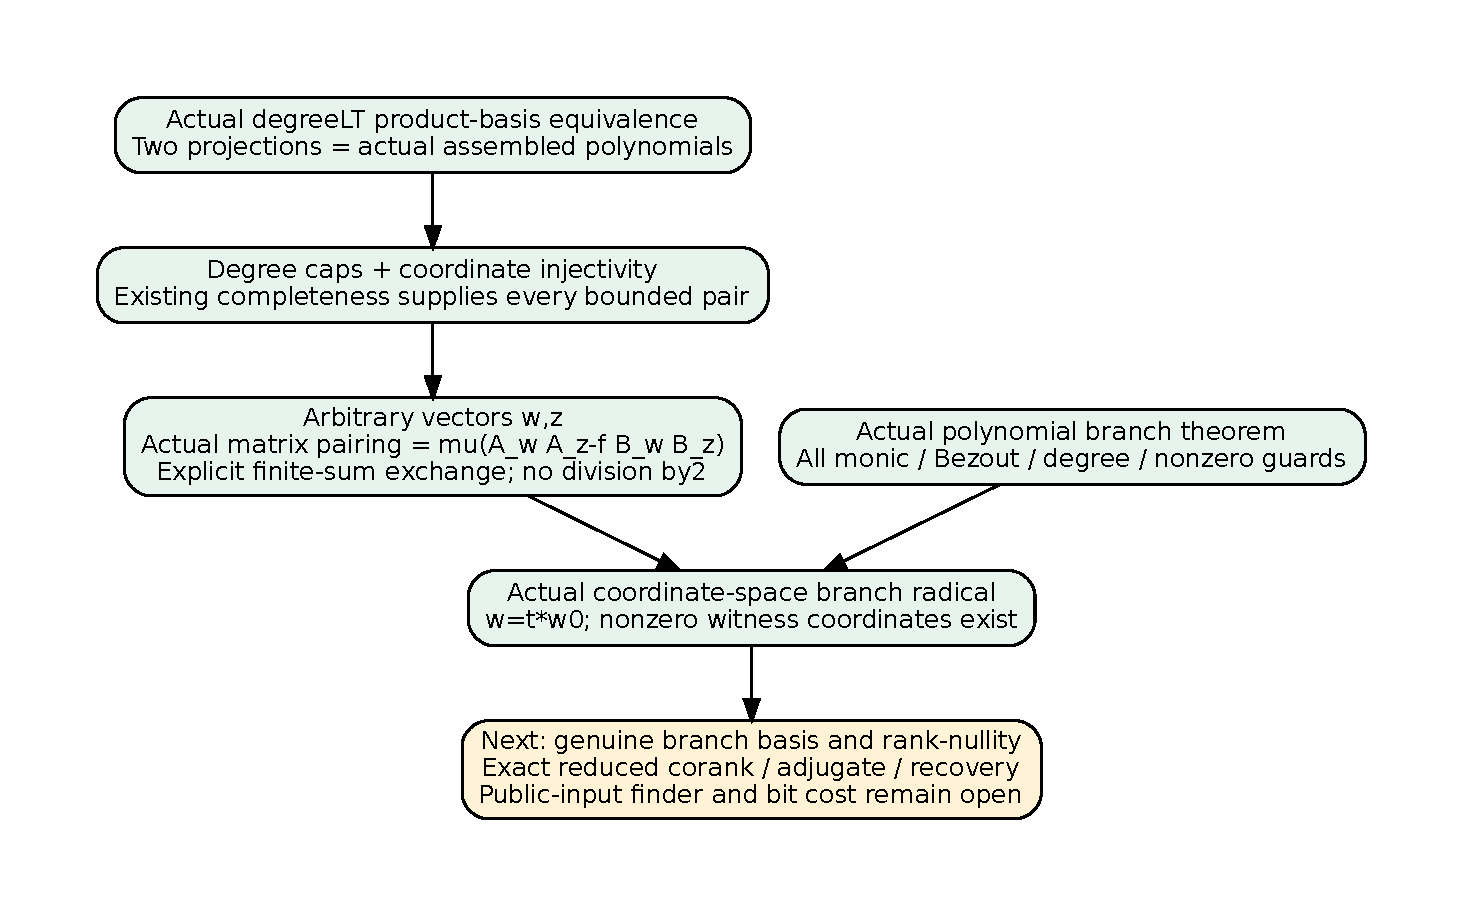
\includegraphics[width=0.98\linewidth,height=0.38\textheight,keepaspectratio]{faithful.pdf}
\end{center}

\newpage
{\Large Evidence, failed attempts and remaining transfer}

\textbf{Scope.} This is the radical of the form restricted to the actual
branch hyperplane. It is not the kernel of the full unrestricted matrix,
whose polynomial radical has two directions. A reduced branch matrix needs a
genuine basis and the remaining rank-nullity/adjugate argument. No rank of an
unrelated matrix is asserted. The supplied witness/Bezout data and moments are
not found by this theorem; a public-input finder and its bit cost remain open.
Jet-family reachability, constant-$H$ and degree-drop charts remain separate.

\textbf{Formal map.} Frozen source \path{d9fddfca0},
\path{NormMatrixFaithful.lean}; ten declarations cover both actual projections,
coordinate injectivity, both assembled degree caps, the arbitrary-vector
polynomial double sum, actual matrix bilinear identity, scalar assembly,
coordinate branch radical and nonzero witness-coordinate existence. Exact
hypotheses and current unsigned PCC bindings accompany the Markdown report.

\textbf{Checks.} Pinned Lean4.35.0, CryptoLean148f5dc, Mathlibcfc55fc.
Builds007/008 complete3151 jobs. The current tracked-source gate and fresh
import-inclusive replay have attributable completion receipts; no additional
trusted axiom is admitted. All producer standing remains unsigned.

\textbf{Failures retained.} Draft002 fails on exchanged summation indices;
the diagonal would conceal the mismatch. An explicit sum exchange fixes003.
Draft004 fails on scalar smul versus field multiplication;005 fixes it.
Draft006 adds nonzero witness coordinates. Failed logs are preserved.

The initial ten unsigned PCC bindings were appended before their preservation
audit exposed a lookup collision: the maintained tool matches theorem short
names, so new lowerDegree shadowed an older theorem despite distinct Lean
namespaces. Older source was unchanged. Unique new assembled-degree names
restore current and earlier bindings. Two replacement claims, original files,
append-only ledger entries and an explanatory note are retained. No signed
verdict is invented. Fresh001 was stopped with143 before the rename; it is not
a pass. Fresh002 checks the renamed frozen source.

\textbf{Sources.} Pinned Mathlib Basis.equivFun/equivFun\_symm\_apply and
actual degreeLT product basis; existing assembly/moment-matrix definitions,
actual polynomial branch theorem and continuation plans. Standard basis/form
transfer, no priority claim. KB MCP/wrapper unavailable; bounded fallback.
Primary summation-polynomial context remains Galbraith15.8.1--2, source-pinned
in the adjacent cost audit.

\textbf{Next.} Choose a genuine basis of the actual branch kernel, identify
the reduced matrix kernel with the nonzero witness line, derive exact corank
and a nonzero adjugate, then supply every guarded recovery hypothesis.

\textbf{Resources.} Local proof correctness only; no mathematical Python
research, new paid job or timing/scaling campaign. Python was used only for
maintained PCC administration. Monthly isolab budget remains exhausted.
No benchmark, leaderboard or ecdb edit. Canonical measured figures remain
unchanged. Editable DOT/SVG and exact receipts accompany this report.
\end{document}
